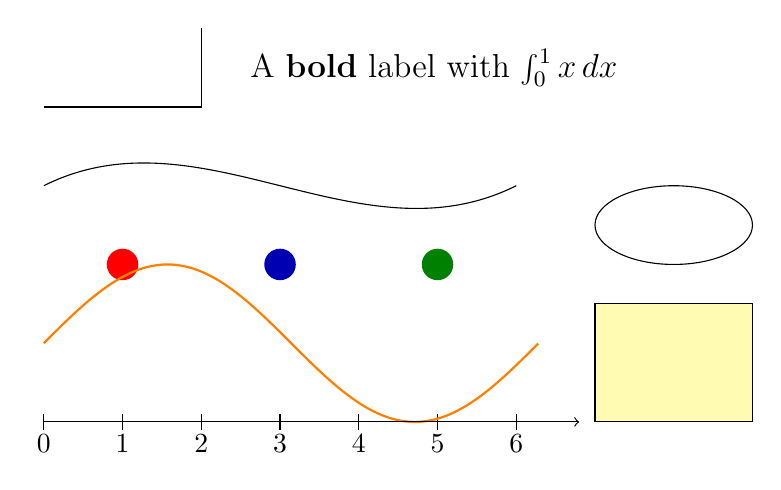
\begin{tikzpicture}
  \foreach \x in {0,1,...,6} { \draw (\x,-0.1) -- (\x,0.1) node[below=4pt] {\x}; }
  \foreach \x/\c in {1/red, 3/blue!70!black, 5/green!50!black} { \fill[\c] (\x, 2) circle (0.2); }
  \draw[domain=0:6.28, samples=80, smooth, orange, thick] plot (\x, {sin(\x r) + 1});
  \draw[->] (0,0) -- (6.8,0);
  \draw (0,3) .. controls (2,4) and (4,2) .. (6,3);
  \draw[fill=yellow!30, draw=black] (7,0) rectangle (9,1.5);
  \draw (8,2.5) ellipse (1 and 0.5);
  \draw (0,4) -| (2,5);
  \node[font=\large, anchor=west] at (2.5,4.5) {A \textbf{bold} label with $\int_0^1 x\,dx$};
\end{tikzpicture}
